\documentclass[12pt]{article}
\usepackage[a4paper,top=1.3cm,bottom=2cm,left=1.5cm,right=1.5cm,marginparwidth=0.75cm]{geometry}
\usepackage{setspace}
\usepackage{cmap}	
\usepackage{graphics}				
\usepackage{mathtext} 	
\usepackage[T2A]{fontenc}			
\usepackage[utf8]{inputenc}		
\usepackage[english,russian]{babel}
\usepackage{tikz}
\usepackage[colorlinks=true, urlcolor=blue, linkcolor=blue]{hyperref}

\usepackage{tabularx}
\usepackage{tabularray} 

\title{CollectorA \\ Brief Description}

\begin{document}
\maketitle

\section*{Цели создания}
Для разработки архитектуры основного проекта (A project) требуется весьма точный расчёт нагрузок на систему. 
Для этого необходимо собрать информацию с уже существующих социальных сетей. \\

Часть информации о трафике использования доступна через общедоступные источники со статистикой, такие как Similar Web. 
Таким образом можно получить информацию о нагрузке на чтение данных с платформы, например: в среднем просмотр страниц Instagram длится 8:39 минут, 
5.7млрд посещений платформы за последний месяц, за раз просмотрено в среднем 11.66 станиц. Отсюда можно вычислить среднюю нагрузку на чтение: 
$5.7 * 10^9 * 11.66 / (30 * 24 * 3600) = 25641$ (в среднем) запросов на чтение в секунду при 1.44млрд пользователей по всему миру.\\

Пиковую нагрузку нужно ещё подумать, как можно вычислить.\\

Но для информации о нагрузке на загрузку данных в БД подходящих источников не найдено.\\

По этой причине было сделано решение о создании сборщика информации CollectorA. Он будет собирать следующие данные:
\begin{enumerate}
    \item Запись id-имя
    \item Кол-во подписок
    \item Кол-во подписчиков
    \item Пробег по последним 10 постам
        \begin {enumerate}
            \item Среднее кол-во лайков
            \item Среднее кол-во комментов
            \item Среднее кол-во репостов
            \item Средний размер записей (сами записи не сохраняются)
            \item Частота выкладывания постов ((10я-1я)/10)
        \end{enumerate}
\end{enumerate}

Располагая соответствующей информацией о достаточно большом количестве пользователей можно вычислить 
среднее и пиковое значения нагрузок на загрузку данных в БД. \\

Дополнительно, можно будет примерно вычислить необходимое количество
места на серверах под одного пользователя. Тем самым предположить ёмкость БД, необходимый для работы системы.\\

Помимо этого, можно будет получить ещё \textit{некоторую} информацию из этих данных другими аналитическими методами.\\

\textit{Булочка: получим опыт в разработке приложений.}

\section*{Основные функции}
Собирает данные с нескольких социальных сетей (Instagram, Facebook, Twitter), вытаскивает из них нужное и записывает в БД.

\section*{Схема работы}
Для каждой соц. сети будет свой сервер, который занимается сбором данных, т. е. отправляет запрос, получает данные 
с веб-сервера и достаёт из них нужную информацию. Далее эти данные отправляются к серверу, которые занимается записью в БД, ну и потом,
соответственно, в базу данных.\\

\textit{Примечание: под "сервером" в данном случае подразумевается один или несколько Java-class-ов , а не как отдельно стоящая вычислительная машина.} 

\begin{figure}[!h]
    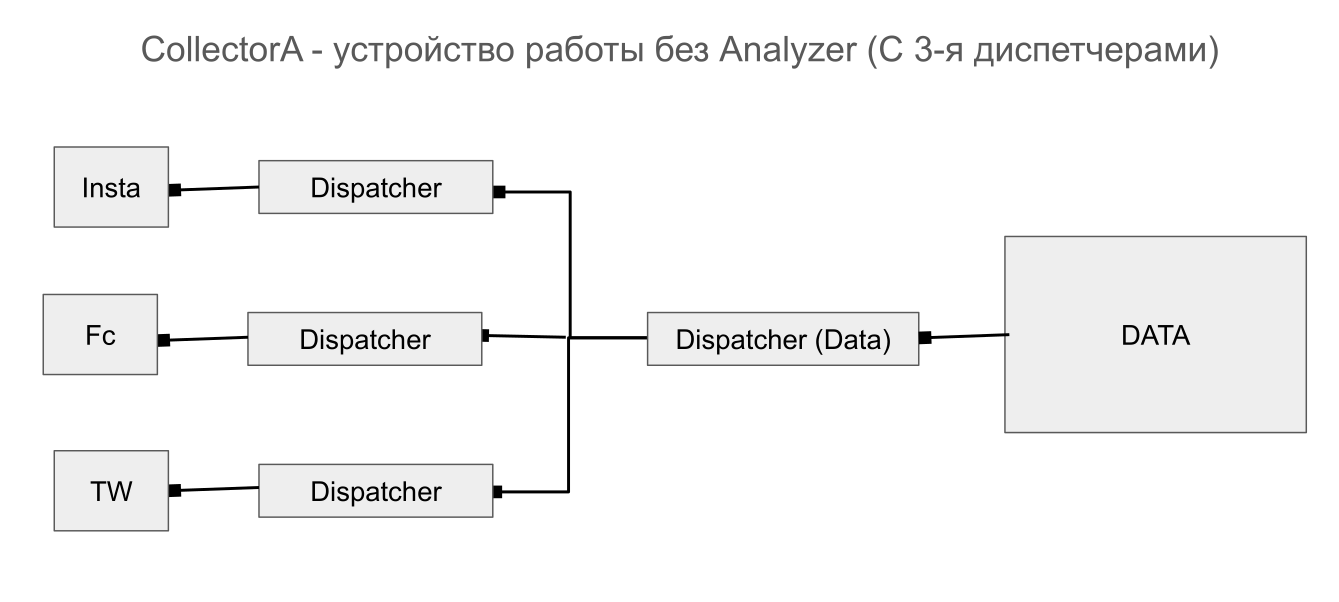
\includegraphics[width=\linewidth]{Scheme.png}
\end{figure}

\section*{Инструменты}
\subsection*{База данных}
Apache Cassandra.\\
Повторю своё сообщение из нашего чата telegram: \textit{"PostgreSQL достаточного в данном случае, но в крупных проектах, 
где необходимо использование распределённых систем, реляционные базы данных уже теряют свои преимущества. 
Поэтому мы хотели поучиться  использовать (набрать опыт в использовании) Apache Cassandra, которая отлично подходит 
для больших проектов и распределённых систем."}

\subsection*{Фреймфорк}
Spring без Spring Boot или Spring Boot? \\
Повторю сообщение из telegtam: \textit{"Хочу сразу спросить: насколько вообще хорошо использовать Spring Boot вместо Spring Framework? 
Да, я знаю, что Spring Boot - это просто "надстройка" над Spring Framework.
По идее он упрощает разработку, но при этом может скрывать какие-то детали. Насколько это критично? 
Не лучше ли использовать обычный Spring Framework с тонкой настройкой?"}

\subsection*{Формат пакетирования приложения}
Скорее всего .jar хватит для данного приложения. Если есть советы - буду рад услышать, потому что в интернете очень размытая информация)

\end{document}